\documentclass[twocolumn]{article}

\usepackage{amsmath}
\usepackage{amsthm}
\usepackage[hidelinks]{hyperref}
\hypersetup{
  pdftitle={The Absorptive Capacity Gap in AI Adoption: A Segmented, Stage-Based Explanation from Two Developer Surveys},
  pdfauthor={Lars Malmqvist},
}
\usepackage{graphicx}
\usepackage{authblk}
\usepackage[margin=1.2cm]{geometry}
\usepackage{natbib}
\usepackage{booktabs}
\usepackage{xcolor}

% Bibliography style: numbered, sorted
\bibliographystyle{chronnat}
\setcitestyle{numbers,square}

\graphicspath{{../figures/}}

\begin{document}

\title{\textbf{The Absorptive Capacity Gap in AI Adoption: A Segmented, Stage-Based Explanation from Two Developer Surveys}}

\author[1]{Lars Malmqvist}
\affil[1]{Research and Implementation ApS, Copenhagen, Denmark\protect\\ \textit{Email: lars@resai.dk}}
\date{}

\setcounter{Maxaffil}{0}
\renewcommand\Affilfont{\itshape\small}

\maketitle

\begin{abstract}
\noindent This paper explains why individual AI tool usage is widespread while organisational AI adoption maturity and confidence in AI outputs remain limited. We analyse the 2026 Practical Data Community State of Data Engineering Survey ($n{=}1{,}101$) and triangulate with the 2025 Stack Overflow Developer Survey ($n{=}49{,}191$). In the Practical Data sample, 82.2\% of respondents use AI daily or more, yet only 23.5\% report adoption beyond experimentation. Among daily+ users, 38.9\% report that their organisation is still experimenting or has no meaningful adoption, a ``Shadow AI'' segment. Constraints shift by maturity stage: organisational bottlenecks dominate early stages while technical constraints dominate among embedded organisations. In multivariate models within daily+ users, unclear data ownership and ad-hoc data modelling are the strongest correlates (by average marginal effect) of Shadow AI status, consistent with an absorptive-capacity interpretation in which social integration mechanisms enable conversion from potential to realised capability. The Stack Overflow data exhibits a parallel usage--trust gap: 64.8\% use AI tools weekly or more, but only 32.8\% trust AI output accuracy. Among daily users, distrust is associated with debugging overhead (OR $\approx 2.49$) and shallow integration (copilot-only vs daily agent use, OR $\approx 2.04$). Together, the surveys suggest that AI adoption is constrained less by tool access than by the organisational routines that cut verification costs, stabilise semantics, and assign accountability.
\end{abstract}


\section{Purpose and contributions}

AI tools have spread quickly through technical work. In the Practical Data survey, 82.2\% of respondents use AI daily or more, but only 23.5\% say AI is embedded in workflows or backed by internal AI platforms. The correlation between individual usage frequency and organisational adoption maturity is positive but weak (Spearman $\rho{=}0.203$). Frequent use, by itself, does not produce mature adoption.

The paper extracts explanatory leverage from two recent survey instruments and makes three contributions with direct practical implications. First, it identifies and sizes a ``Shadow AI'' segment (high-frequency users whose organisations have not moved beyond experimentation), giving managers a concrete metric (the adoption-efficiency proxy) for diagnosing conversion failure. Second, it treats adoption maturity as a stage-based conversion problem and documents a bottleneck inversion in which organisational constraints dominate early stages and technical scaling constraints dominate later ones, implying that interventions must be matched to maturity stage rather than applied uniformly. Third, it triangulates the maturity gap with a parallel usage--trust gap in Stack Overflow and ties distrust to integration depth and verification costs, suggesting that trust is built through infrastructure rather than mandates.


\section{Theoretical background}

Cohen and Levinthal~\cite{cohen1990absorptive} defined absorptive capacity as a firm's ability to recognise external knowledge, assimilate it, and put it to commercial use. Zahra and George~\cite{zahra2002absorptive} split it into potential absorptive capacity (PACAP), covering acquisition and assimilation, and realised absorptive capacity (RACAP), covering transformation into operational routines. The conversion from PACAP to RACAP turns on social integration mechanisms: the formal and informal structures through which knowledge is shared, interpreted, and built into organisational action. Jansen et al.~\cite{jansen2005managing} showed empirically that coordination capabilities track with PACAP while socialisation capabilities (connectedness, shared coding schemes) track with RACAP. Lane et al.~\cite{lane2006reification} called for research that pinpoints where in the assimilation-to-exploitation pipeline organisations get stuck, rather than treating absorptive capacity as a static asset.

The IS literature has a parallel concept: the assimilation gap. Fichman and Kemerer~\cite{fichman1999illusory} showed that IT innovations spread fast in acquisition but slowly in routine deployment, especially for ``knowledge barrier'' innovations~\cite{fichman2004real} requiring complementary organisational changes. Tornatzky and Fleischer's~\cite{tornatzky1990processes} TOE framework predicts the same: technologies demanding new governance and accountability structures will show a persistent gap between individual uptake and organisational embedding.

\subsection{The AI-specific adoption problem}

Recent work sharpens these predictions for AI. Brynjolfsson et al.~\cite{brynjolfsson2021productivity} formalise a Productivity J-Curve: general-purpose technologies demand large upfront investments in intangible capital before productivity gains appear. Brynjolfsson et al.~\cite{brynjolfsson2023generative} confirm the pattern: generative AI raises productivity, but gains depend on deployment context, not access alone. Berente et al.~\cite{berente2021managing} frame AI management around inscrutability and output unpredictability. Pumplun et al.~\cite{pumplun2023organizational} find that most organisations stall at experimentation because they lack routines for handling probabilistic, opaque outputs at scale.

Trust adds another dimension. Glikson and Woolley~\cite{glikson2020human} find that trust depends on the transparency of AI outputs. Jussupow et al.~\cite{jussupow2024algorithm} model algorithm aversion as shaped by verification costs and explanatory infrastructure. On the governance side, Waters-Lynch et al.~\cite{frey2024shadow} introduce ``shadow user innovation'' for employees deploying generative AI without approval, creating individual value but stalling organisational learning, while Raisch and Krakowski~\cite{raisch2021artificial} identify an automation--augmentation paradox requiring design choices that correspond to social integration mechanisms. Dell'Acqua et al.~\cite{dellacqua2023navigating} provide experimental evidence of a ``jagged technological frontier'' where AI fails unpredictably. Lebovitz et al.~\cite{lebovitz2022maintain} find the same among radiologists.

Taken together, this literature points to a structural conversion problem. The gap between AI tool access (PACAP) and organisational embedding (RACAP) depends on investments in governance, shared semantics, and evaluation routines. We ask whether two large survey datasets reveal patterns consistent with this view.

We use the PACAP/RACAP distinction as an \textit{analytic lens} rather than claiming to measure absorptive capacity directly. Individual AI usage frequency serves as a proxy for the ``potential'' side (access to and experimentation with external knowledge), while organisational maturity stage proxies the ``realised'' side (routinised exploitation). Data ownership and modelling practices are interpreted as proxies for social integration mechanisms. These mappings involve measurement error (absorptive capacity is an organisational-level construct and our measures are individual-level self-reports), but they provide a theoretically grounded vocabulary for interpreting the observed gaps.


\section{Data and method}

\subsection{Datasets}

The primary dataset is the 2026 Practical Data Community State of Data Engineering Survey ($n{=}1{,}101$)~\cite{practicaldata2026}. It captures individual AI usage frequency (five-level ordinal: Never, Rarely, Weekly, Daily, Multiple times per day), organisational AI adoption maturity on a five-stage ordinal scale (No meaningful adoption yet, Experimenting, Using AI for tactical tasks, Building internal AI platforms, AI embedded in most workflows), data modelling approach (free text, coded into eight categories), modelling pain points (multi-select), biggest bottleneck (single-select), and organisational context (role, industry, organisation size, region, expected team growth). The secondary dataset is the 2025 Stack Overflow Developer Survey ($n{=}49{,}191$)~\cite{stackoverflow2025}, which we use to triangulate on AI usage frequency, trust in AI accuracy, measured on a five-point scale from Highly trust to Highly distrust, AI agent usage depth, and reported frustrations.

The two surveys have different sampling frames and question wordings: Practical Data draws from a data-engineering community, Stack Overflow from a broad developer population. We use the second dataset for \textit{pattern replication} (testing whether the gap structure recurs in an independent sample) rather than for quantitative comparability of point estimates. Stack Overflow's published methodology reports 49,009 qualified responses, but the public microdata file contains 49,191 rows. Our analyses use the microdata directly. Question-specific response counts are smaller (AI frequency: $n{=}33{,}720$, AI accuracy trust: $n{=}33{,}297$) because not all respondents answered every item.

\subsection{Construct definitions}

We derive three constructs from the Practical Data survey:

\begin{itemize}
\item \textbf{Beyond experimentation}: organisations at \textit{Building internal AI platforms} or \textit{AI embedded in most workflows} (the top two stages). The middle stage (\textit{Using AI for tactical tasks}) is deliberately excluded: tactical use may not reflect the routinised, governance-backed embedding that absorptive-capacity theory associates with RACAP.
\item \textbf{Shadow AI}: respondents who use AI tools daily or more \textit{and} whose organisation is at \textit{Experimenting} or \textit{No meaningful adoption yet}. We use ``shadow'' not in the narrow sense of covert or policy-violating use (which we do not measure), but in the broader sense of high-frequency individual use that occurs outside routinised organisational embedding and visibility, consistent with the ``shadow user innovation'' framing of Waters-Lynch et al.~\cite{frey2024shadow}. Where measurement-precise language is needed, we refer to this as the ``high-use/low-maturity segment.''
\item \textbf{Adoption-efficiency proxy}: the ratio of respondents beyond experimentation to respondents using AI daily or more ($=23.5/82.2 \approx 0.29$). This provides a coarse gauge of how much individual-level usage converts into organisational embedding.
\end{itemize}

\subsection{Missing data and variable coding}

In the Practical Data survey no variables used in the analysis have missing values ($n{=}1{,}101$ complete cases). The role field is free-text. We grouped responses into eight categories: Data Engineer (reference), Manager/Director/VP, Analytics Engineer, Data Architect, Software Engineer, Platform Engineer, ML/AI Engineer, and Other (roles with $n{<}10$). Organisation size has five levels (reference: 1,000--9,999 employees), industry has six (reference: Financial services), and team growth expectations has four (reference: Grow). Modelling approach was recoded from free text into eight categories (reference: Mixed). Bottleneck type was classified as Organisational, Technical, or Other (reference: Technical) based on survey-provided response options. ``Organisational'' includes Lack of leadership direction, Poor requirements/upstream issues, and Talent/hiring. ``Technical'' includes Legacy/technical debt, Data quality, Compute costs, and Tool complexity. Modelling pain-point flags are binary indicators for each multi-select option.

In the Stack Overflow survey, we restrict to respondents with non-missing AI accuracy trust ($n{=}33{,}297$). For the distrust model, we further filter to daily AI tool users and exclude neutral trust responses (analysis $n{=}11{,}321$). Agent-bucket ``Other'' and ``Missing'' categories were excluded due to ambiguous interpretation. Organisation size missing values ($n{=}2{,}193$) are coded as a separate ``Missing'' category rather than dropped, to preserve sample size. Reference categories are Agents daily (agent bucket) and 1,000--4,999 employees (organisation size).

\subsection{Statistical approach}

We use cross-tabulations and Spearman rank correlation to characterise the adoption gap descriptively. To assess which factors remain associated with Shadow AI status after adjusting for correlated organisational context, we estimate logistic regressions and report average marginal effects (AME) with 95\% confidence intervals. Model fit is evaluated via McFadden pseudo-$R^{2}$ (the proportional reduction in log-likelihood relative to the intercept-only model), AIC, and BIC. Statistical significance is assessed at $\alpha{=}0.05$ using Wald tests on individual coefficients.

\textbf{Model 1 (Practical Data)}: Logistic regression within daily+ users ($n{=}905$), with Shadow AI as the binary outcome. Predictors: modelling approach, four modelling pain-point indicators, bottleneck type, organisation size, industry, role (grouped), and team growth expectations (33 parameters). Estimation via Newton--Raphson. McFadden pseudo-$R^{2}{=}0.087$, AIC${=}1{,}170$, BIC${=}1{,}329$. Model converged.

\textbf{Model 2 (Stack Overflow)}: Logistic regression among daily AI users excluding neutral trust responses ($n{=}11{,}321$), with distrust as the binary outcome. Predictors: agent-usage depth, three frustration indicators, and organisation size (18 parameters). Estimation via BFGS. McFadden pseudo-$R^{2}{=}0.071$, AIC${=}13{,}719$, BIC${=}13{,}841$. Standard errors are based on the observed information matrix.

Both models are cross-sectional and associative. We do not claim causal identification. Full coefficient tables and reproducibility code are publicly available.\footnote{Reproducibility materials (code, variable codebooks, and full model outputs) are archived at \url{https://github.com/lmlearning/cade_2026}.}


\section{Results}

\subsection{Baseline distributions (Practical Data)}

Figure~\ref{fig:usage_adoption} shows usage and adoption maturity in the Practical Data sample. Usage is heavily right-skewed: 28\% report daily use, 54\% multiple times per day. Organisational maturity clusters in experimentation (31\%) and tactical adoption (34\%), with 14\% building platforms and 10\% embedded.

\begin{figure}[t]
\centering
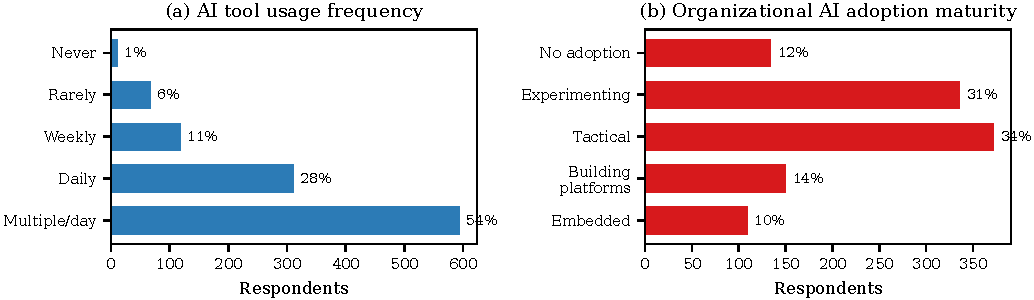
\includegraphics[width=\columnwidth]{fig1_usage_and_adoption.pdf}
\caption{AI tool usage frequency and organisational AI adoption maturity (Practical Data, $n{=}1{,}101$).}
\label{fig:usage_adoption}
\end{figure}


\subsection{The Shadow AI segment}

In the full sample, 82.2\% report daily+ AI use while only 23.5\% report adoption beyond experimentation, for an adoption-efficiency proxy of 0.29 (${=}23.5/82.2$). The gap is not driven by low-usage respondents. Shadow AI accounts for 32.0\% of the full sample. Within the daily+ subset ($n{=}905$), 38.9\% say their organisation is still experimenting or has no meaningful adoption.

Figure~\ref{fig:shadow_ai} breaks out organisational maturity within daily+ users and weekly-or-less users. The daily+ group is more mature on average, but a large minority sits in experimentation or no adoption, which is why the usage--maturity correlation stays weak even in a population where daily use is the norm.

\begin{figure}[t]
\centering
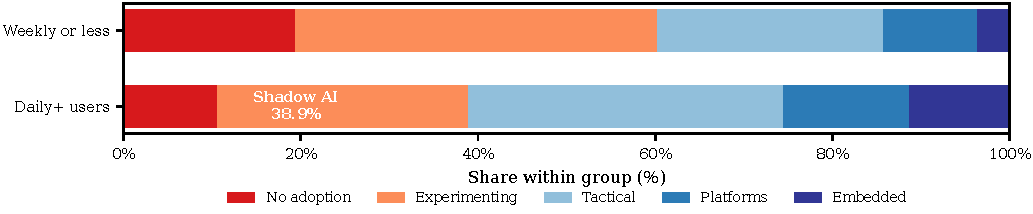
\includegraphics[width=\columnwidth]{fig2_shadow_ai_segmentation.pdf}
\caption{Adoption-stage distribution within usage groups. Shadow AI is daily+ use with organisation at experimentation or below.}
\label{fig:shadow_ai}
\end{figure}


\subsection{Bottleneck inversion across maturity stages}

Reported constraints shift by maturity stage (Figure~\ref{fig:bottleneck}). We classify bottlenecks using the survey's response options: ``organisational'' groups Lack of leadership direction, Poor requirements/upstream issues, and Talent/hiring. ``Technical'' groups Legacy/technical debt, Data quality, Compute costs, and Tool complexity. At no adoption, 60.4\% cite organisational bottlenecks versus 37.3\% technical. At embedded maturity, the ratio flips: 50.5\% technical, 41.3\% organisational. The pattern fits a stage model in which early progress depends on social integration mechanisms (direction, ownership, routinisation) and later progress depends on the underlying data and systems being able to scale.

\begin{figure}[t]
\centering
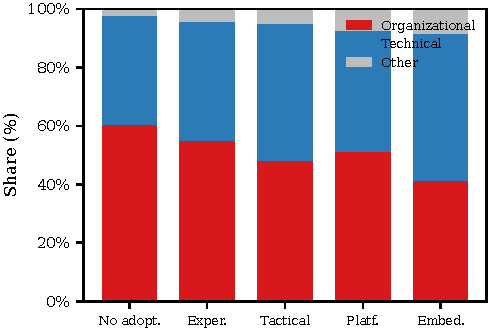
\includegraphics[width=\columnwidth]{fig3_bottleneck_inversion.pdf}
\caption{Bottleneck inversion: early stages over-index on organisational constraints. Embedded organisations over-index on technical constraints.}
\label{fig:bottleneck}
\end{figure}


\subsection{Data modelling and maturity}

Ad-hoc modelling drops sharply with maturity: 25.4\% at no adoption, 9.2\% at embedded. More informative is what replaces it. Embedded organisations do not converge on one modelling formalism. Mixed approaches are the most common category at 48.6\%. The differentiator appears to be the presence of explicit, shared semantics, often hybrid, rather than allegiance to any single school.

\begin{figure}[t]
\centering
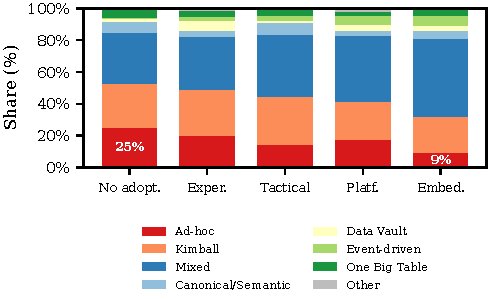
\includegraphics[width=\columnwidth]{fig4_modeling_mix.pdf}
\caption{Modelling approach mix by adoption stage. The strongest monotone signal is the decline in ad-hoc modelling.}
\label{fig:modeling_mix}
\end{figure}


\subsection{Predictors of Shadow AI among daily+ users}

Model~1 is a logistic regression within daily+ users ($n{=}905$, McFadden pseudo-$R^{2}{=}0.087$) with controls for organisation size, industry, role, growth expectations, modelling approach, bottleneck type, and modelling pain points. Figure~\ref{fig:predictors} reports average marginal effects (AME) for selected predictors, and Table~\ref{tab:model1} gives the corresponding odds ratios.

Unclear ownership has the largest average marginal effect among the substantive predictors (OR${=}1.77$, 95\% CI $[1.32, 2.37]$, $p{<}0.001$), associated with a ${+}12.0$ percentage-point increase in the probability of Shadow AI. Ad-hoc modelling adds ${+}11.7$ pp (OR${=}1.74$, $[1.14, 2.64]$, $p{=}0.009$). Data Vault modelling has the largest OR in Table~\ref{tab:model1} (OR${=}2.25$), but this category has few observations and the confidence interval is wide. The ownership and ad-hoc modelling effects are large relative to a 38.9\% baseline rate. Respondents in large organisations (${\geq}10{,}000$ employees) are less likely to fall into the Shadow AI segment (OR${=}0.54$, $[0.35, 0.83]$, $p{=}0.005$), plausibly because size correlates with governance investment. Organisational bottleneck has a positive but non-significant association (OR${=}1.24$, $[0.92, 1.66]$, $p{=}0.16$). The estimates are cross-sectional and associative, but they line up with the claim that codified knowledge structures and defined accountability are the social integration mechanisms that matter most for the PACAP-to-RACAP conversion.

\begin{table}[t]
\centering
\small
\caption{Model 1: Key predictors of Shadow AI (logistic regression, daily+ users, $n{=}905$). Reference categories: Mixed (modelling), Technical (bottleneck), Data Engineer (role), 1,000--9,999 (org size). McFadden pseudo-$R^{2}{=}0.087$.}
\label{tab:model1}
\begin{tabular}{@{}lrrr@{}}
\toprule
Predictor & OR & 95\% CI & $p$ \\
\midrule
Unclear ownership (pain) & 1.77 & [1.32, 2.37] & ${<}.001$ \\
Ad-hoc modelling (vs mixed) & 1.74 & [1.14, 2.64] & .009 \\
Data Vault (vs mixed) & 2.25 & [1.03, 4.90] & .042 \\
Org bottleneck (vs technical) & 1.24 & [0.92, 1.66] & .160 \\
Org size $\geq$10,000 (vs 1,000--9,999) & 0.54 & [0.35, 0.83] & .005 \\
Manager/VP (vs Data Eng) & 0.57 & [0.38, 0.86] & .007 \\
Growth: stay same (vs grow) & 1.55 & [1.13, 2.12] & .006 \\
\bottomrule
\end{tabular}
\end{table}

\begin{figure}[t]
\centering
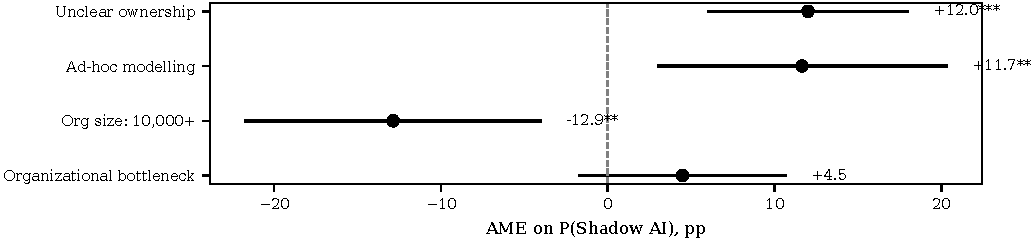
\includegraphics[width=\columnwidth]{fig5_shadow_ai_predictors.pdf}
\caption{Key predictors of Shadow AI among daily+ users (average marginal effects with controls). Significance: {*}\,$p{<}.05$, {**}\,$p{<}.01$, {***}\,$p{<}.001$ (Wald test).}
\label{fig:predictors}
\end{figure}


\subsection{Triangulation: the Stack Overflow usage--trust gap}

Stack Overflow shows a parallel pattern: 64.8\% use AI tools weekly or more, but only 32.8\% trust AI output accuracy and 45.7\% actively distrust it. Among daily users, distrust is patterned. Daily agent users have a distrust share of 18.9\%. Among respondents who do not plan to use agents, the share is 40.3\%.

Model~2 is a logistic regression among daily AI tool users excluding neutral trust responses ($n{=}11{,}321$, McFadden pseudo-$R^{2}{=}0.071$). Debugging overhead is the strongest frustration correlate (OR${=}2.49$, 95\% CI $[2.29, 2.71]$, $p{<}0.001$). Copilot-only users are roughly twice as likely to distrust as daily agent users (OR${=}2.04$, $[1.80, 2.32]$), and those who do not plan to use agents are 3.5$\times$ as likely (OR${=}3.51$, $[3.11, 3.97]$). These associations may partly reflect reverse causality (trust enabling deeper use) or omitted variables such as organisational support that facilitates both agent adoption and trust. The cross-sectional design cannot distinguish these pathways, but the pattern is consistent with the absorptive-capacity interpretation: deeper integration reduces per-output verification costs, which supports cognitive trust formation.

\begin{figure}[t]
\centering
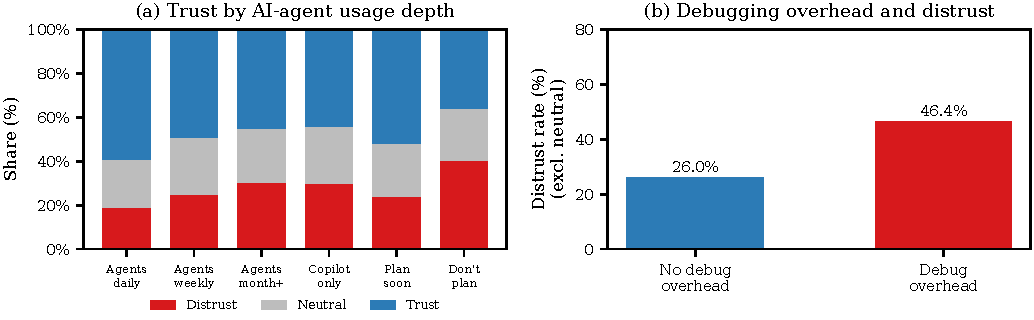
\includegraphics[width=\columnwidth]{fig6_so_trust_mechanism.pdf}
\caption{Trust correlates among daily AI tool users: agent depth and debugging overhead (Stack Overflow 2025).}
\label{fig:trust_mechanism}
\end{figure}

\begin{figure}[t]
\centering
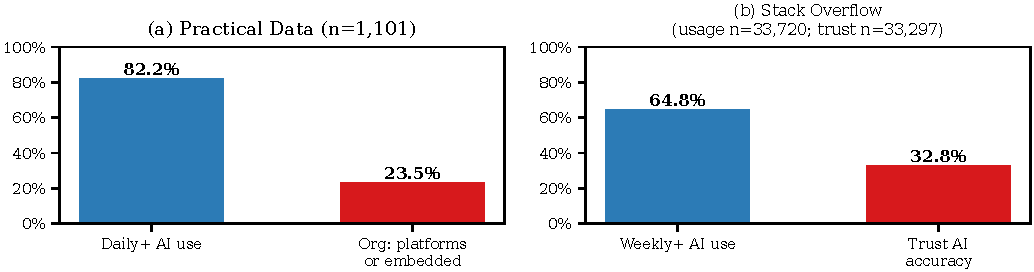
\includegraphics[width=\columnwidth]{fig7_dual_survey_gaps.pdf}
\caption{Two adoption gaps: usage vs organisational maturity (Practical Data) and usage vs trust (Stack Overflow). Question-specific response Ns differ from the full survey N (see text).}
\label{fig:dual_gaps}
\end{figure}


\section{Discussion}

The two surveys document the same structural asymmetry from different angles. PACAP is cheap. RACAP is expensive. The absorptive capacity framework predicts exactly this for knowledge-barrier innovations, and the pattern is consistent with the Productivity J-Curve~\cite{brynjolfsson2021productivity}: these organisations are in the investment phase, building governance structures that do not yet register as measured output.

The high-use/low-maturity segment anchors the abstract claim. Nearly two in five daily AI users work in organisations that have not moved beyond experimentation. These are heavy users in organisations lacking the integration mechanisms to convert experimentation into accountable workflows. The logistic model picks out two structural correlates: unclear data ownership and ad-hoc data modelling. Both correspond to what Zahra and George~\cite{zahra2002absorptive} call social integration mechanisms. The pattern maps onto recognisable sector-specific dynamics: in supply-chain analytics, demand-forecasting models trained on inconsistently owned inventory data produce predictions that no single team is accountable for validating. In healthcare, clinical decision-support tools built without shared diagnostic ontologies generate outputs that clinicians cannot reconcile with institutional protocols. In both cases individual tool use is high but organisational embedding stalls for want of the same codified semantics and ownership structures surfaced by our model. The ownership and modelling variables hold up after controls for organisation size, industry, and growth expectations, suggesting explanatory weight independent of organisational demographics.

The bottleneck inversion adds a stage-dependent dimension. Early-stage organisations are stuck on coordination failures (direction, requirements, talent), while embedded organisations face technical scaling constraints (legacy, data quality, compute). Fichman~\cite{fichman2004real} and the TOE framework~\cite{tornatzky1990processes} predict that adoption barriers change character as organisations move from acquisition to deployment.

The Stack Overflow trust findings point to a complementary mechanism. Distrust among daily users tracks integration depth and verification costs, mapping onto the jagged frontier of Dell'Acqua et al.~\cite{dellacqua2023navigating}. The agent-depth/distrust association may reflect reverse causality, and the two surveys differ in sampling frame, so the triangulation's value lies in structural recurrence, not matched magnitudes. Jussupow et al.'s~\cite{jussupow2024algorithm} framework predicts that high verification costs push users toward aversion. Glikson and Woolley's~\cite{glikson2020human} cognitive trust distinction suggests the mechanism runs through reliability assessment.

The finding fits a broader pattern. Waters-Lynch et al.~\cite{frey2024shadow} argue that unmanaged generative AI use creates individual value but stalls organisational learning. Raisch and Krakowski's~\cite{raisch2021artificial} automation--augmentation paradox applies: the same tool that boosts individual output can undermine coordination when its use is unmanaged. In practice, the PACAP-to-RACAP pathway runs through three observable steps: first, individual experimentation creates local know-how (PACAP acquisition). Second, teams codify what works into shared artefacts (data contracts, evaluation rubrics, prompt libraries) that make AI outputs interpretable across roles (social integration). Third, governance structures assign accountability for AI-assisted decisions, enabling routinised use (RACAP). Our data suggest most organisations stall between the first and second steps: individuals use AI heavily, but the codification and ownership investments that would make outputs organisationally legible have not been made.


\section{Managerial implications}

Measure conversion, not procurement. An adoption-efficiency proxy, defined as the share of respondents whose organisations are at platform or embedded stages divided by the share of respondents using AI daily or more, sits at roughly 0.29 in this dataset. Tracking this ratio over time across business units is more informative than counting tool licences or training completions. If the ratio stays flat while usage grows, PACAP is piling up without converting.

Match interventions to the stage of the bottleneck. For organisations stuck in the high-use/low-maturity segment, the binding constraint is social integration: explicit ownership for data domains, stable upstream contracts, shared semantic artefacts. Concretely, ``explicit ownership'' means assigning named domain owners accountable for data definitions, quality, and access policies. ``Shared semantic artefacts'' means documented data models, semantic layers, or data contracts that codify how entities and metrics are defined, creating the shared codebook through which AI outputs become organisational rather than individual. For organisations already building platforms, the constraint shifts to technical scaling: paying down legacy debt, improving data quality infrastructure, controlling production costs.

Treat distrust as a diagnostic, not as resistance. When developers say that debugging AI output costs more time than it saves, the right response is to ask which grounding artefacts are missing, not to mandate more AI usage. Deeper integration (agent-level rather than copilot-only) correlates with lower distrust in the Stack Overflow data, but that association probably reflects the organisational infrastructure that makes deeper integration viable, not the tool depth itself.

A minimal governance framework for PACAP-to-RACAP conversion should address three layers: \textit{semantic} (data contracts and shared definitions that make AI outputs interpretable), \textit{accountability} (named domain owners responsible for validating and acting on AI-assisted decisions), and \textit{evaluation} (lightweight feedback loops, including output spot-checks, accuracy tracking, and escalation protocols, that reduce per-output verification costs over time). Organisations that invest in all three layers create the social integration mechanisms that absorptive capacity theory identifies as the conversion bottleneck. Crucially, the gap narrows fastest when these investments are sequenced: codify semantics first (so AI outputs become comparable), assign ownership second (so someone is accountable for acting on them), and build evaluation infrastructure last (so verification costs fall with each iteration rather than remaining constant).


\section{Limitations and future work}

Both surveys are cross-sectional, observational, and drawn from self-selected technical communities. The associations should not be read as causal and may not generalise to non-technical populations. The logistic models have modest explanatory power (pseudo-$R^{2}$ of 0.087 and 0.071), and key constructs (adoption maturity, modelling pain points, bottleneck type) are single self-report items. Our ``Shadow AI'' construct captures a usage--maturity mismatch but does not measure whether use is covert or policy-violating. Multi-item instruments designed around the PACAP/RACAP distinction~\cite{jansen2005managing,flatten2011measure} would allow sharper tests.

Three directions seem worth pursuing: longitudinal data to test whether ownership and modelling changes precede maturity gains, linkage to operational indicators (data quality metrics, semantic coverage, deployment frequency), and extension to non-technical populations where the gap may take a different shape.


\bibliography{references}

\end{document}
